% Uncomment this to make slides with overlays:
%\documentclass[slides]{beamer}

% Uncomment these (but comment the above \documentclass line) to make handouts:
\documentclass[handout]{beamer}

% Uncomment these to have more than one slide per page
\usepackage{pgfpages}
\pgfpagesuselayout{2 on 1}[border shrink=5mm]
\pgfpageslogicalpageoptions{1}{border code=\pgfusepath{stroke}}
\pgfpageslogicalpageoptions{2}{border code=\pgfusepath{stroke}}

\usepackage[]{graphicx, color, hyperref}

\mode<presentation>
{
	%\usetheme[secheader]{Boadilla}
	%\usecolortheme[rgb={.835, .102,.169}]{structure}  
	\usetheme[width= 0cm]{Goettingen}
	%\setbeamercovered{transparent}
}
\setbeamertemplate{navigation symbols}{}
\setbeamertemplate{footline}[frame number]

\definecolor{blue2}{rgb}{0.278,0.278,0.729} 
\newcommand{\blue}[1]{\textcolor{blue2}{#1}}
\newcommand{\white}[1]{\textcolor{white}{#1}}
\newcommand{\red}[1]{\textcolor{red}{#1}}
\newcommand{\xbar}{\overline{x}}
\newcommand{\ybar}{\overline{y}}
\newcommand{\phat}{\widehat{p}}
\newcommand{\prob}{\mbox{Pr}}
\newcommand{\E}{\mathbb{E}}
\newcommand{\Var}{\mbox{Var}}
\newcommand{\cp}{\oplus}
\newcommand{\cm}{\circleddash}

\title{Lecture 16: Sample Size and Power}
\author{Chapter 4.6}
\date{}


\begin{document}
%------------------------------------------------------------------------------
\begin{frame}
\titlepage
\end{frame}
%------------------------------------------------------------------------------


%-------------------------------------------------------------------------------
\begin{frame}
\frametitle{Last Time:  Reedie Sleep Example}
Tested number of hours of sleep:
\begin{itemize}
\item $H_0: \mu = 7$
\item $H_A: \mu > 7$
\end{itemize}

\vspace{3cm}

\end{frame}
%-------------------------------------------------------------------------------


%-------------------------------------------------------------------------------
\begin{frame}
\frametitle{Two-Sided Alternative Hypothesis}
Say instead we had a \blue{two-sided alternative hypothesis}:

\begin{itemize}
\item $H_0: \mu = 7$
\item $H_A: \mu \neq 7$
\end{itemize}

\pause The the p-value would be double: $2 \times 0.007= 0.014$.  Picture:

\begin{center}
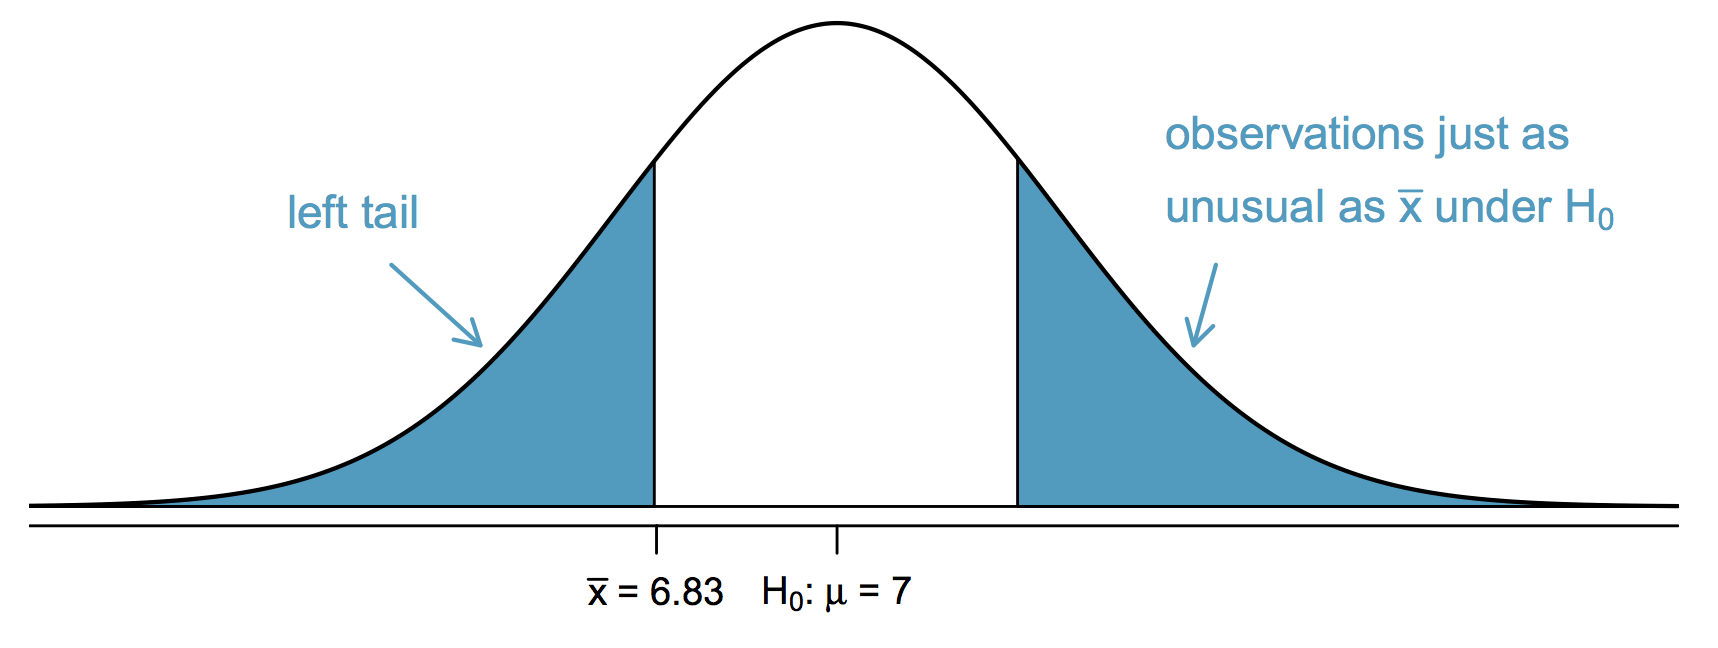
\includegraphics[width=\textwidth]{figure/two-sided.png}
\end{center}

\end{frame}
%-------------------------------------------------------------------------------


%------------------------------------------------------------------------------
\begin{frame}[fragile]
\frametitle{Setting $\alpha$}

Say Dr. Quack is conducting a hypothesis tests.  They start with $\alpha=0.05$.

\pause\vspace{0.5cm}

They conduct the test and get \blue{p-value = 0.09}.  They then declare ``having used an \blue{$\alpha=0.10$}, we reject the null hypothesis and declare our results to be significant.''

\pause\vspace{0.5cm}
What's not honest about this approach?

\pause\vspace{0.5cm}
Ronald Fisher, the creator of p-values, never intended for them to be used this way:  \blue{\href{http://en.wikipedia.org/wiki/P-value\#Criticisms}{http://en.wikipedia.org/wiki/P-value\#Criticisms}}

\end{frame}
%------------------------------------------------------------------------------


%------------------------------------------------------------------------------
\begin{frame}[fragile]
\frametitle{Goals for Today}

\begin{itemize}
\item More in depth discussion of 
\begin{itemize}
\item 10\% sampling rule
\item Skew condition to check to use the normal model
\end{itemize}
\item How big a sample size do I need?
\item Statistical power
\item Statistical vs practical significance
\end{itemize}

\end{frame}
%------------------------------------------------------------------------------


%------------------------------------------------------------------------------
\begin{frame}[fragile]
\frametitle{10\% Sampling Rule}

\blue{Question}: Why do we set $n$ to be less than 10\% of the population size $N?$

\pause\vspace{0.5cm}

\blue{Intuition}: Shouldn't we always sample as many people as we can?

\pause\vspace{0.5cm}

\blue{Answer}: Yes, if we only care about the mean.  If we also care about the SE, then we need to be careful.  

\pause\vspace{0.5cm}

\blue{Explanation}:  Recall from HW5 Q1, sampling without replacement from a rooms that are half male/female but with $N=10$ and $N=10000$.  

\end{frame}
%------------------------------------------------------------------------------


%------------------------------------------------------------------------------
\begin{frame}[fragile]
\frametitle{Finite Population Correction}

%
% Comment this
%
The \blue{finite population correction (FPC)} to the SE accounts for the \blue{sampling without replacement}:
\[
SE = \frac{\sigma}{\sqrt{n}} \times \blue{\sqrt{\frac{N-n}{N-1}}} =
\frac{\sigma}{\sqrt{n}} \times \blue{FPC}
\]
Say we have $N=10000$.  
\begin{itemize}
\pause\item Let $n=100$ (1\%), then
\[
FPC=\sqrt{\frac{10000-100}{10000-1}} = 0.995
\]
\pause\item Let $n=5000$ (50\%), then
\[
FPC=\sqrt{\frac{10000-5000}{10000-1}} = 0.707
\]
\end{itemize}

\end{frame}
%------------------------------------------------------------------------------


%------------------------------------------------------------------------------
\begin{frame}[fragile]
\frametitle{Finite Population Correction}
%
% Comment this
%

\[
SE = \frac{\sigma}{\sqrt{n}} \times \blue{\sqrt{\frac{N-n}{N-1}}} =
\frac{\sigma}{\sqrt{n}} \times \blue{FPC}
\]

\vspace{0.25cm}
\pause
We've been ignoring the \blue{FPC}.  So when 
\begin{itemize}
\pause\item $n$ is relatively small, the FPC $\approx$ 1, so not a problem.
\pause\item $n$ is relatively large, the FPC $\longrightarrow$ 0.\\
i.e. $\frac{\sigma}{\sqrt{n}}$ is not the true SE.  
\end{itemize}

\vspace{0.25cm}
\pause Conclusion:  By capping $n \leq $ 10\% of $N$, we have a \blue{rule of thumb} for keeping the FPC ``close'' to 1.  

\end{frame}
%------------------------------------------------------------------------------


%------------------------------------------------------------------------------
\begin{frame}[fragile]
\frametitle{Sampling}
We can tie the \blue{conceptual} and \blue{mathematical} notions of sampling:  

\vspace{0.25cm}
\pause
\blue{Conceptual}:  If we sample everybody, we know the true $\mu$.
\begin{center}
\pause and
\end{center}
\blue{Mathematical}:  
If $n=N$ then $FPC = \sqrt{\frac{N-n}{N-1}} = 0$ then $SE = \frac{\sigma}{\sqrt{n}}\times FPC = 0$


\vspace{0.25cm}
\pause
i.e. 
\begin{itemize}
\item the sampling distribution is just one point: the true $\mu$.
\item if we repeat this procedure many times, we get the same value each time: 0 variability.
\end{itemize}


\end{frame}
%------------------------------------------------------------------------------


%------------------------------------------------------------------------------
\begin{frame}[fragile]
\frametitle{Sampling and the SE}
\blue{Question}:  Why do we care that our SE is correct?

\pause\vspace{0.5cm}

\blue{Answer}:  If not
\begin{itemize}
\item the $SE$ in confidence intervals is off
\item the $z$-scores of $\xbar$ have the wrong denominator
\end{itemize}

\end{frame}
%------------------------------------------------------------------------------


%%------------------------------------------------------------------------------
%\begin{frame}[fragile]
%\frametitle{10\% Sampling Rule} 
%\blue{Example}:  From MATH392 where we sample $n=40,000$ without replacement from a population of size $N=60,000$
%\begin{itemize}
%\item The histogram represents the true sampling distribution
%\item The red curve represents the sampling distribution with the \blue{uncorrected} $SE=\frac{s}{\sqrt{n}}$
%\end{itemize}
%
%\begin{center}
%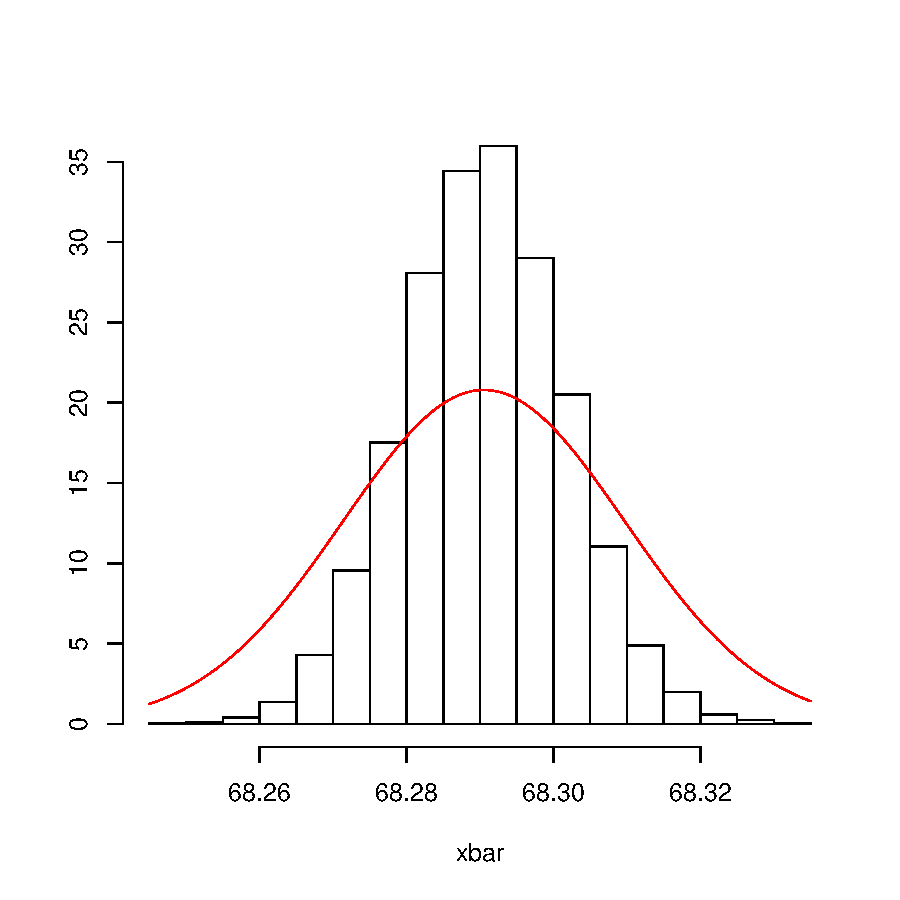
\includegraphics[width=0.55\textwidth]{figure/FPC.pdf}
%\end{center}
%
%\end{frame}
%%------------------------------------------------------------------------------


%------------------------------------------------------------------------------
\begin{frame}
\frametitle{Skew Condition to Check to Use Normal Model}
Throughout the book, they talk about the condition for $\xbar$ being nearly normal and using $s$ in place of $\sigma$ in $SE=\frac{\sigma}{\sqrt{n}}$:

\vspace{0.25cm}

\begin{itemize}
\pause\item On page 164: the population distribution is not strongly skewed
\pause\item On page 167: the data are not strongly skewed
\pause\item On page 168: the distribution of sample observations is not strongly skewed
\pause\item On page 185: the population data are not strongly skewed
\end{itemize}

\end{frame}
%------------------------------------------------------------------------------


%------------------------------------------------------------------------------
\begin{frame}
\frametitle{Skew Condition to Check to Use Normal Model}
However, they all mean the same thing:

\begin{enumerate}
\pause\item The \blue{true population} distribution from which you are drawing your sample observations/data $x_1, \ldots, x_n$ is not too skewed.  
\pause\item The histogram (visual estimate) of the sample observations/data $x_1, \ldots, x_n$ is not too skewed.  
\end{enumerate}

\end{frame}
%------------------------------------------------------------------------------


%------------------------------------------------------------------------------
\begin{frame}
\frametitle{Sample Size:  Thought Experiment}
Say you have two distributions with $\mu=15$ but different $\sigma$.
\begin{center}
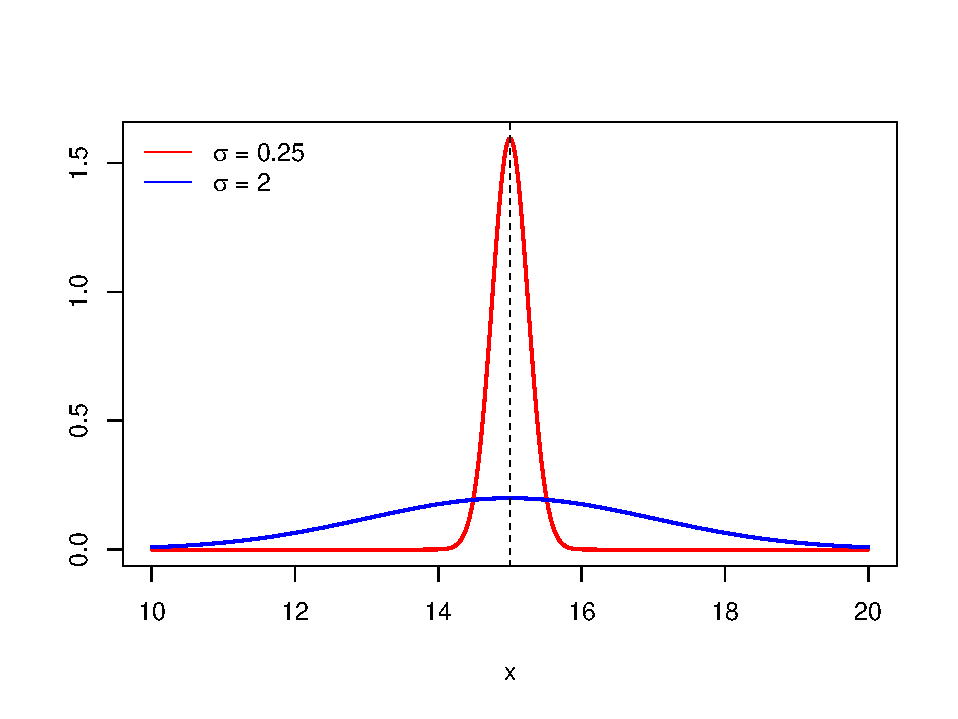
\includegraphics[width=0.75\textwidth]{figure/norm.pdf}
\end{center}
\pause Which of the two distributions do you think will require a bigger $n$ to estimate $\mu$ ``well''?
\end{frame}
%------------------------------------------------------------------------------


%------------------------------------------------------------------------------
\begin{frame}
\frametitle{Margin of Error}
Recall our formula for a 95\% confidence interval:
\[\left[
\overline{x} - 1.96 \frac{s}{\sqrt n}, \mbox{  }
\overline{x} + 1.96 \frac{s}{\sqrt n}
\right]\]

\pause The \blue{margin of error} is half the width of the CI.\\

\vspace{0.25cm}

\pause Say we knew the \blue{true} standard deviation $\sigma$, then
\[
\mbox{Margin of Error = } 1.96 \frac{\sigma}{\sqrt n} 
\]
\end{frame}
%------------------------------------------------------------------------------



%------------------------------------------------------------------------------
\begin{frame}
\frametitle{Identify $n$ for a Desired Margin of Error}
%
% Comment this
%
To estimate the necessary sample size $n$ for a maximum desired margin of error $m$, we set
\[
m \geq z^* \frac{\sigma}{\sqrt{n}}
\]
and solve for $n$.  
\end{frame}
%------------------------------------------------------------------------------


%------------------------------------------------------------------------------
\begin{frame}
\frametitle{Identify $n$ for a Desired Margin of Error}
Since
%
% Comment this
%
\begin{eqnarray*}
&&m \geq z^*\frac{\sigma}{\sqrt{n}}\\
&& \sqrt{n} \geq z^*\frac{\sigma}{m}\\
&& n \geq \left(z^*\frac{\sigma}{m}\right)^2\\
\end{eqnarray*}

\vspace{3cm}

\pause So
\begin{itemize}
\pause\item As $\sigma$ goes up, you need more $n$
\pause\item As $z^*$ goes up, i.e. higher confidence level, you need more $n$
\pause\item As the desired margin of error goes down, you need more $n$
\end{itemize}

\end{frame}
%------------------------------------------------------------------------------


%------------------------------------------------------------------------------
\begin{frame}
\frametitle{Back to Thought Experiment}
For the same desired maximal margin of error $m$ and same confidence level, we need a larger $n$ to estimate the mean of the blue curve:
\begin{center}
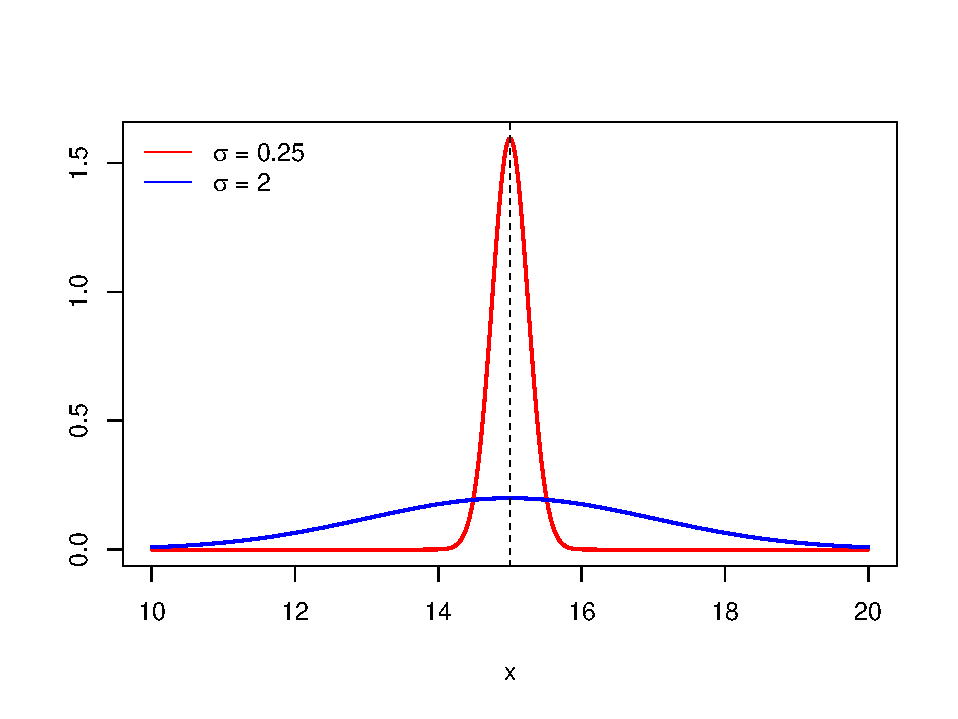
\includegraphics[width=0.8\textwidth]{figure/norm.pdf}
\end{center}
\end{frame}
%------------------------------------------------------------------------------



%-------------------------------------------------------------------------------
\begin{frame}
\frametitle{Type II Error Rate and Power}
%
% Comment this
%
For a hypothesis test:

\begin{itemize}
\item The significance level $\alpha$ is the \blue{type I error rate}:  the rate at which we reject $H_0$ when it is true.
\pause\item The \blue{type II error rate $\beta$} is the rate at which we fail to reject $H_0$ when $H_A$ is true.
\pause\item $1-\beta$ is called the \blue{statistical power}: the rate at which we reject $H_0$ when $H_A$ is true.  
\end{itemize}

\end{frame}
%-------------------------------------------------------------------------------



%-------------------------------------------------------------------------------
\begin{frame}
\frametitle{Type II Error Rate and Power}
%
% Comment this
%
Say we are conducting $N=A+B+C+D$ hypothesis tests.
\pause\begin{center}
  \begin{tabular}{cc|cc}
     \multicolumn{2}{c}{}  & \multicolumn{2}{c}{\textbf{Test conclusion}} \\ 
     &  & do not reject $H_0$ & reject $H_0$ in favor of $H_A$ \\ 
\hline
    \textbf{Truth} & $H_0$ true & A & B \\ 
     & $H_A$ true & C & D \\ 
    \hline
  \end{tabular}
\end{center}

\vspace{0.25cm}

\begin{itemize}
\pause \item The \blue{Type I Error rate} is $\alpha = \frac{B}{A+B}$: rate at which B occurs \blue{given $H_0$ is true}.
\pause \item The \blue{Type II Error} is $\beta = \frac{C}{C+D}$: rate at which 
C occurs \blue{given $H_A$ is true}.
\pause \item The \blue{power} is $1-\beta = 1-\frac{C}{C+D} = \frac{D}{C+D}$: rate at which D occurs \blue{given $H_A$ is true}.
\end{itemize}

\end{frame}
%-------------------------------------------------------------------------------


\end{document}














%x <- seq(5.7, 8.2, by=0.01)
%y <- dnorm(x, 7, 1.75/sqrt(110))
%y1 <- dnorm(x, 7.5, 1.75/sqrt(110))
%
%pdf("./7.2 Sample Size and Power/power1.pdf", width=8*0.8, height=6*0.8)
%plot(x,y,type='l', ylab="", xlab="hours of sleep")
%abline(h=0)
%abline(v=7.274, col="red")
%abline(v=7)
%legend("topleft", 
%       legend=c("Null Value 7",
%                "Rejection Cutoff 7.274"), 
%       lty=c(1,1), 
%       col=c(1,2), bty='n')
%dev.off()
%
%pdf("./7.2 Sample Size and Power/power2.pdf", width=8*0.8, height=6*0.8)
%plot(x,y,type='l', ylab="", xlab="hours of sleep")
%abline(h=0)
%abline(v=7.274, col="red")
%abline(v=7)
%abline(v=7.42, col="blue")
%legend("topleft", 
%       legend=c("Null Value 7",
%                "Rejection Cutoff 7.274",
%                "Observed Xbar 7.42"), 
%       lty=c(1,1,1), 
%       col=c(1,2,"blue"), bty='n')
%dev.off()
%
%pdf("./7.2 Sample Size and Power/power3.pdf", width=8*0.8, height=6*0.8)
%plot(x,y,type='l', ylab="", xlab="hours of sleep")
%lines(x,y1,lty=2)
%abline(h=0)
%abline(v=7.274, col="red")
%abline(v=7)
%abline(v=7.5, lty=2)
%legend("topleft", 
%       legend=c("Null Value 7",
%                "Rejection Cutoff 7.274",
%                "Alternative Mean 7.5"),
%       lty=c(1,1,2), 
%       col=c(1,2,1), bty='n')
%dev.off()
%%-------------------------------------------------------------------------------
%\begin{frame}
%\frametitle{Power}
%Since
%\[
%z = \frac{\xbar - \mbox{null value}}{SE} = \frac{\xbar - 7}{\frac{1.75}{\sqrt{110}}}
%\]
%and since the area to the right of $z=1.64$ is $0.05=\alpha$ we have:
%\[
%z \times SE + \mbox{null value} = 1.64 \times \frac{1.75}{\sqrt{110}} + 7 = 7.274 
%\]
%
%\vspace{0.25cm}
%
%For any observed $\xbar\geq \textcolor{red}{7.274}$, we would reject the null hypothesis!
%
%\end{frame}
%%-------------------------------------------------------------------------------
%
%
%%------------------------------------------------------------------------------
%\begin{frame}
%\frametitle{Power}
%i.e. we reject $H_0$ if $\xbar$ falls to the right of the \textcolor{red}{red} line.  
%\begin{center}
%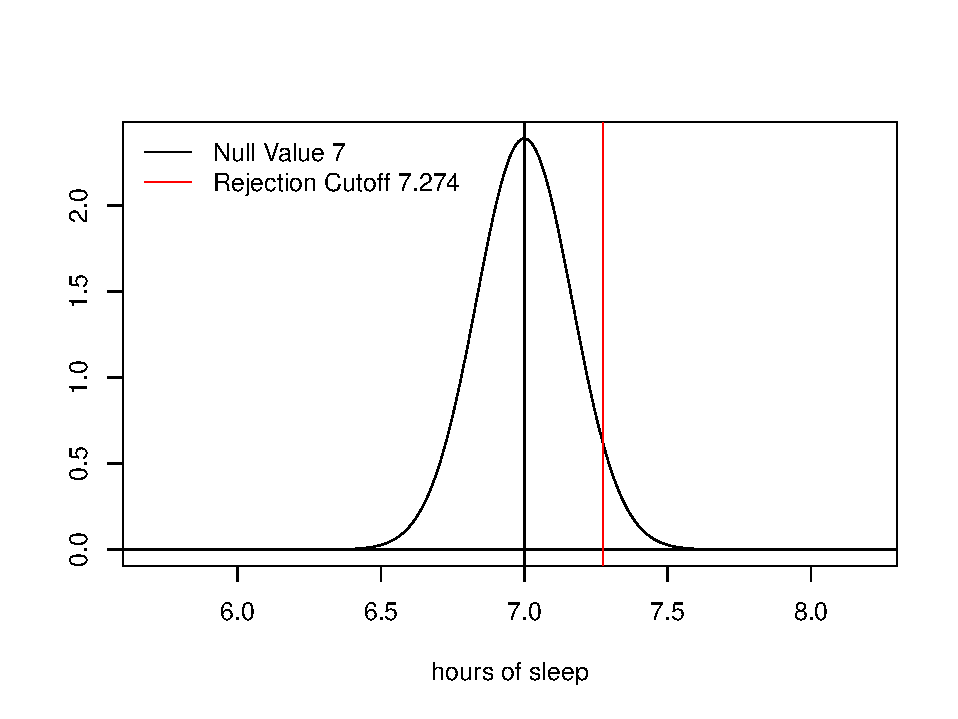
\includegraphics[width=0.95\textwidth]{figure/power1.pdf}
%\end{center}
%\end{frame}
%%------------------------------------------------------------------------------
%
%
%%------------------------------------------------------------------------------
%\begin{frame}
%\frametitle{Power}
%For example, since we observed $\xbar=\textcolor{blue}{7.42}$, we rejected $H_0$. 
%\begin{center}
%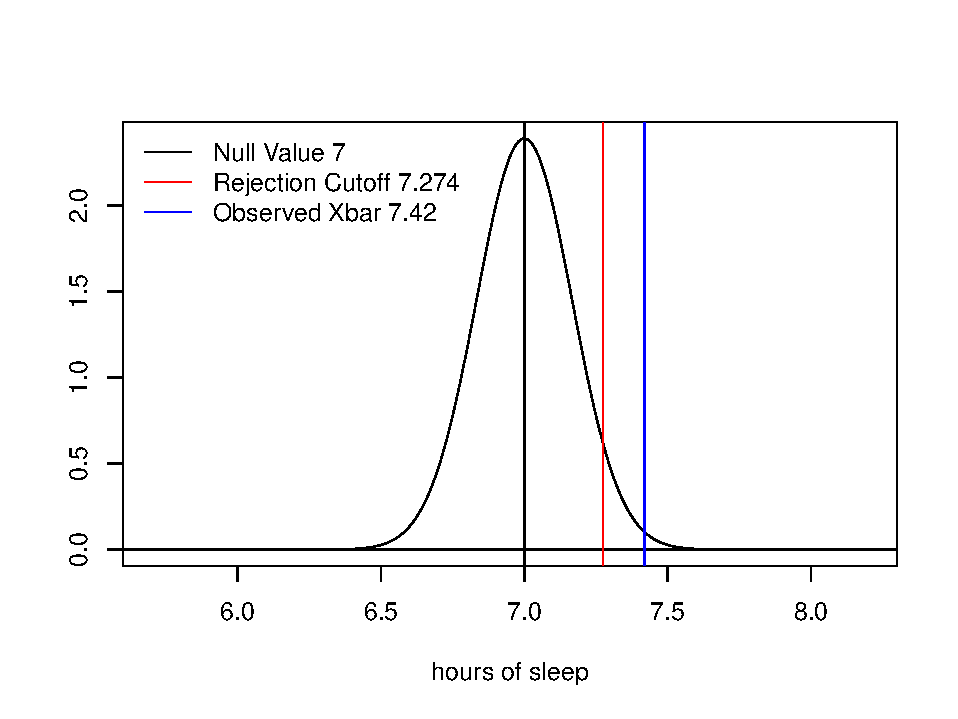
\includegraphics[width=0.95\textwidth]{figure/power2.pdf}
%\end{center}
%\end{frame}
%%------------------------------------------------------------------------------
%
%
%%-------------------------------------------------------------------------------
%\begin{frame}
%\frametitle{Power}
%Now say we had an alternative hypothesis that was true, specifically $\mu = 7.5$.  
%
%\vspace{0.5cm}
%
%Given our rejection threshold: reject $H_0$ if $\xbar>\textcolor{red}{7.274}$, what is the power? 
%
%\vspace{0.5cm}
%
%What is Power = P(Rejecting $H_0$ when $H_A$ is true)?
%
%\end{frame}
%%-------------------------------------------------------------------------------
%
%
%%------------------------------------------------------------------------------
%\begin{frame}
%\frametitle{Power}
%\textcolor{white}{The power is the prop'n of the dashed line normal curve is to the right of the red line.}
%\begin{center}
%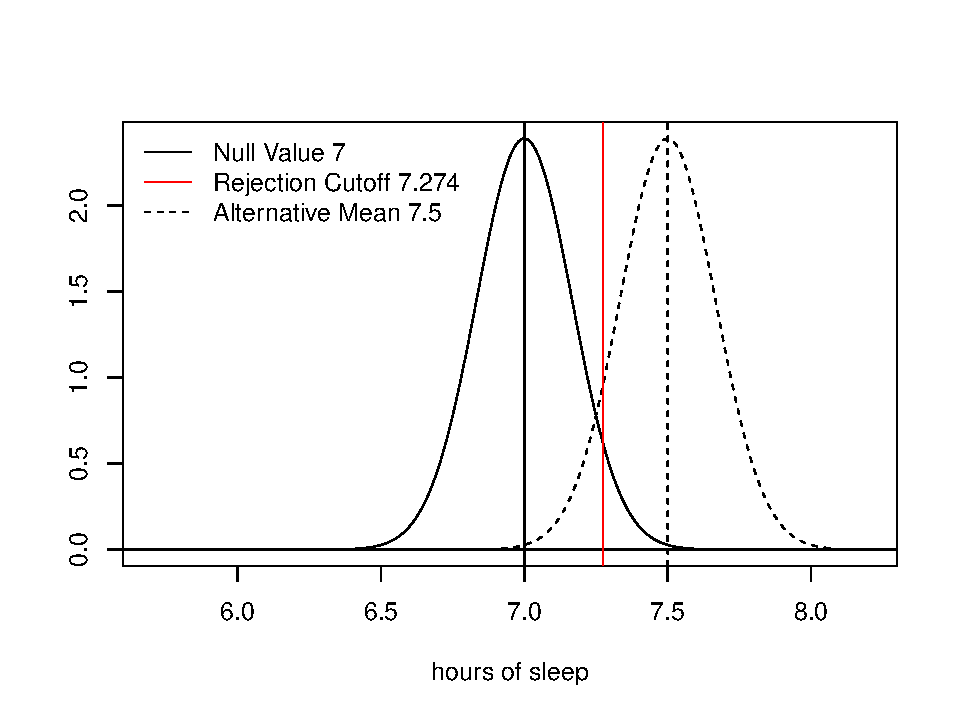
\includegraphics[width=0.95\textwidth]{figure/power3.pdf}
%\end{center}
%\end{frame}
%%------------------------------------------------------------------------------
%
%
%%------------------------------------------------------------------------------
%\begin{frame}
%\frametitle{Power}
%The power is the prop'n of the dashed line normal curve is to the right of the \textcolor{red}{red} line.
%\begin{center}
%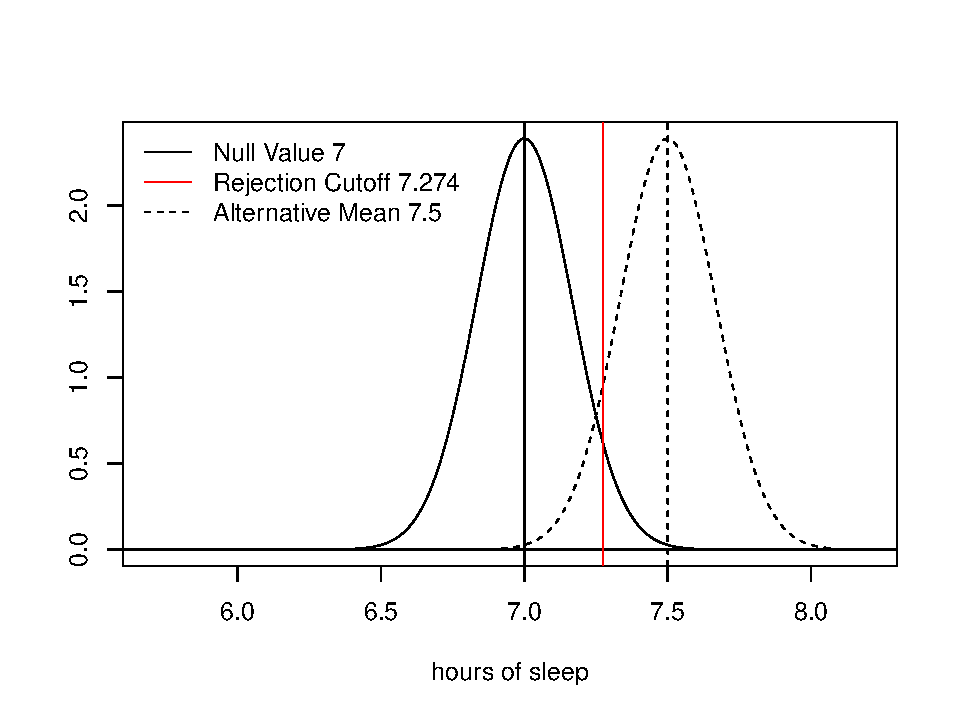
\includegraphics[width=0.95\textwidth]{figure/power3.pdf}
%\end{center}
%\end{frame}
%%------------------------------------------------------------------------------






